\documentclass[11pt]{article}

\usepackage[margin=1in]{geometry}
\usepackage{graphicx}
\usepackage{grffile}
\usepackage{float}
\usepackage{enumitem}
\usepackage{hyperref}
\usepackage{caption}
\usepackage{subcaption}
\usepackage{booktabs}
\usepackage{tabularx}
\usepackage{url}
\makeatletter
\renewcommand{\maketitle}{%
  \begin{center}
    {\LARGE\bfseries\@title\par}
    \vspace{0.35em}
    {\large\@author\par}
    \vspace{0.2em}
    {\normalsize\@date\par}
  \end{center}
  \vspace{0.5em}
}
\makeatother
\makeatletter
\renewcommand\section{\@startsection{section}{1}{\z@}%
  {-2.0ex \@plus -0.4ex \@minus -.2ex}%
  {0.65ex \@plus .15ex}%
  {\normalfont\Large\bfseries}}
\renewcommand\subsection{\@startsection{subsection}{2}{\z@}%
  {-1.35ex \@plus -0.35ex \@minus -.15ex}%
  {0.5ex \@plus .12ex}%
  {\normalfont\large\bfseries}}
\makeatother
\setlength{\floatsep}{6pt plus 2pt minus 2pt}
\setlength{\textfloatsep}{8pt plus 2pt minus 3pt}
\setlength{\intextsep}{8pt plus 2pt minus 2pt}
\captionsetup{skip=5pt, font=small}

\graphicspath{{images/}}

\title{DSA301 Project 4:}
\author{Mustafa Bozyel --- 32417}
\date{}

\newcommand{\strengths}{\paragraph{Design strengths.}}
\newcommand{\weaknesses}{\paragraph{Design weaknesses.}}

\begin{document}

\maketitle
\vspace{-1.25em}

\section{Introduction}

\noindent This document has three parts. \textbf{Part~1A} analyzes historical airline timetables as dense, print-era data visualizations. \textbf{Part~1B} redesigns the Pan Am August 1963 eastbound round-the-world timetable as a map-based sketch. \textbf{Part~2} designs two static Turkish Airlines timetable visualizations that combine map-based and time-based components, with Gestalt-based critiques. \textbf{Part~3} implements an interactive timetable dashboard (\texttt{thy-dashboard.html}) following Shneiderman's overview--filter--detail model, with a written reflection below.

%==============================================================================
\section{Part 1A: Historical Timetable Design Critique}
%==============================================================================

For each carrier we identify design strengths (clarity, hierarchy, encoding) and weaknesses (clutter, ambiguity, cognitive load). Where a route map accompanies the timetable, the map is included for geographic context; the critique focuses on the \textbf{timetable} pages. Pan Am is placed last in Part~1A so that its critique leads directly into the Part~1B map redesign.

%------------------------------------------------------------------------------
\subsection{Singapore Airlines --- December 1, 1972}
%------------------------------------------------------------------------------

\begin{figure}[H]
  \centering
  \includegraphics[width=0.58\textwidth]{{Singapore Airlines - December 1- 1972-route.png}}
  \caption{Singapore Airlines international route map (December 1972 timetable). Included for network context; critique below addresses the timetable.}
  \label{fig:sia-route}
\end{figure}

\begin{figure}[H]
  \centering
  \includegraphics[width=\textwidth]{{Singapore Airlines - December 1- 1972-timetable.png}}
  \caption{Singapore Airlines international flights (December 1972). Pages 24--25: northbound (Table 1) and southbound (Table 2).}
  \label{fig:sia-timetable}
\end{figure}

\subsection{Route map}

The route map uses a high-contrast \textbf{yellow field}, \textbf{olive landmass silhouettes}, and \textbf{black} nodes and edges---a strong mid-century brand palette. Singapore reads as a hub through line density (starburst). Strengths include minimalist geography (topology over borders) and immediate legibility of the title hierarchy. Weaknesses include overlapping arcs in Southeast Asia, unclear distinction between direct and multi-stop services in Europe, and abstract coastlines that offer little orientation beyond city labels.

\subsection{Timetable critique}

\strengths
\begin{itemize}
  \item \textbf{Encoding of flight paths:} Each service is a \textbf{white vertical bar} on a yellow ground---an unusually effective ``small multiple'' within one table: the bar is the flight, and times sit on its endpoints and stops.
  \item \textbf{Hierarchy:} Bold \emph{International flights}, split \emph{NORTHBOUND}/\emph{SOUTHBOUND}, and per-column headers (days, SQ number, aircraft, FY class) guide a top-down search before local reading.
  \item \textbf{Compact symbology:} Meal codes (B, C, D, L, M, R) and downward arrows encode ancillary facts without extra columns; \# marks government-approval caveats inline.
  \item \textbf{Time-zone column:} GMT offsets beside cities support mental conversion; footnotes clarify local times, DST changes (1972), and traffic-right restrictions between city pairs.
\end{itemize}

\weaknesses
\begin{itemize}
  \item \textbf{Cognitive load:} Yellow-on-black at high density fatigues the eye; users must scan horizontally for the correct flight/day, then vertically along a bar---two demanding axes with few full-width grid lines.
  \item \textbf{Clutter at scale:} Many parallel bars on one page resemble a bar chart without margins; adjacent columns compete, especially where bars are short (regional hops).
  \item \textbf{Ambiguity of duration:} All times are local; GMT offsets help experts but do not show block time or ground time between stops without manual calculation.
  \item \textbf{Small secondary marks:} Meal letters and approval symbols are easy to miss at print size, increasing the risk of misreading service level or operability.
\end{itemize}

%------------------------------------------------------------------------------
\subsection{Lufthansa --- April 1--27, 1968}
%------------------------------------------------------------------------------

\begin{figure}[H]
  \centering
  \includegraphics[width=\textwidth]{{lufthansa April 1 1968-route.png}}
  \caption{Lufthansa world route network (\emph{Welt-Streckennetz}, April 1968). Solid lines: jet routes; dotted: connecting routes. City numbers reference timetable tables.}
  \label{fig:lufthansa-route}
\end{figure}

\begin{figure}[H]
  \centering
  \includegraphics[width=\textwidth]{{lufthansa April 1 1968-timetable.png}}
  \caption{Lufthansa Europe--North America timetable (April 1--27, 1968). Outbound (left) and inbound (right) on pale blue stock.}
  \label{fig:lufthansa-timetable}
\end{figure}

\subsection{Route map}

The map is \textbf{monochrome}: black routes and labels on light cyan paper. Solid vs.\ dotted line styles distinguish jet routes from connecting services; numbered cities link to timetable tables---a strong cross-reference encoding. Weaknesses mirror other hub maps: line spaghetti in Europe and the Middle East, uniform line weight (no frequency or distance channel), and crowded numeric labels in dense regions.

\subsection{Timetable critique}

\strengths
\begin{itemize}
  \item \textbf{Grid clarity:} Strict rows (cities) and columns (individual flights) with bold city names support tracing one LH/AF service through many stops. Feeder sections (German cities to hubs) are separated from transatlantic blocks.
  \item \textbf{Efficient encoding:} Stylized aircraft icons, F/Y class tags, and \textbf{circled weekday numbers} (1--7) compress metadata into column headers without prose.
  \item \textbf{Hierarchy:} Trilingual section title (\emph{Nordamerika / North America / Amérique du Nord}) and outbound/inbound page pairing mirror mental models of origin vs.\ return planning.
  \item \textbf{Footnote system:} Geometric symbols in cells point to detailed notes---a standard airline pattern that keeps the grid visually regular while allowing exceptions.
\end{itemize}

\weaknesses
\begin{itemize}
  \item \textbf{Clutter:} Dozens of columns across two pages produce a busy field; feeder flights at top/bottom require long vertical eye travel to connect with main oceanic services.
  \item \textbf{Cognitive load:} Symbol-heavy cells force constant lookup to footnotes---high working-memory cost for occasional travelers.
  \item \textbf{Readability:} Stacked hour/minute in single cells and small type on tinted paper lower contrast compared with black on white; misreads of 13:30 vs.\ 1:30 are more likely.
  \item \textbf{Ambiguity of through-service:} Vertical arrows suggest continuation but do not always distinguish stop vs.\ technical stop vs.\ change of gauge without reading notes.
\end{itemize}

%------------------------------------------------------------------------------
\subsection{Thai Airways International --- July 31, 1960}
%------------------------------------------------------------------------------

\begin{figure}[H]
  \centering
  \includegraphics[width=\textwidth]{{tahi airways july 31 1960-timetable.png}}
  \caption{Thai Airways International timetable (effective July 31, 1960). Tokyo--Calcutta corridor and regional Bangkok--Phnom Penh--Saigon service.}
  \label{fig:thai-timetable}
\end{figure}

\subsection{Timetable critique}

\strengths
\begin{itemize}
  \item \textbf{Hierarchy:} Dark blue header bars with white route strings segment the spread into outbound Tokyo--Calcutta, inbound return, and a smaller regional table---clear chunks before detail.
  \item \textbf{Eye-tracking aids:} Dotted horizontal guides from city names on the margins into the data columns reduce row-tracking error on wide tables---a thoughtful affordance for print.
  \item \textbf{Symbol encoding:} F/T class squares, meal (cutlery) icons, and airplane glyphs convey class and service without extra text; 24-hour times with spaced digits match international norms.
  \item \textbf{Symmetry:} Mirrored city labels on left and right of the main grids support reading from either page edge in a bound booklet.
\end{itemize}

\weaknesses
\begin{itemize}
  \item \textbf{Ambiguity:} The header \emph{Singapore/Rangoon} splits one logical corridor---some columns stop at Singapore, others at Rangoon, marked by dots vs.\ times; easy to misread without careful column-by-column checking.
  \item \textbf{Missing local legend:} X marks, arrow variants, and icon meanings on this spread are not defined here---users must find a global legend elsewhere in the booklet.
  \item \textbf{Clutter in regional table:} The Bangkok--Phnom Penh--Saigon \emph{v.v.} layout packs bidirectional flows into one grid, with dense arrows and times harder to parse than the main Tokyo--Calcutta blocks.
  \item \textbf{Cognitive load:} Promotional DC-6B art and SAS partnership copy compete with schedule data for attention; the center gutter where two large tables meet is especially visually noisy.
\end{itemize}

%------------------------------------------------------------------------------
\subsection{Pan American World Airways --- August 1--31, 1963}
%------------------------------------------------------------------------------

\begin{figure}[H]
  \centering
  \includegraphics[width=\textwidth]{{PanAM August 1, 1963-timetable.png}}
  \caption{Pan Am round-the-world services timetable (August 1--31, 1963). Pages 6--7: eastbound (Table 1) and westbound (Table 2).}
  \label{fig:panam-timetable}
\end{figure}

\subsection{Timetable critique}

\strengths
\begin{itemize}
  \item \textbf{Hierarchy:} A saturated blue header bar, bold \emph{EASTBOUND}/\emph{WESTBOUND} labels, and mirrored page numbers establish direction and brand before the reader enters the grid. The repeated instruction \emph{Read Down} encodes the primary scanning axis explicitly.
  \item \textbf{Encoding consistency:} Rows follow geography (cities with Ar/Lv sub-rows); columns group by day, class (FY), flight number, and aircraft type (JET highlighted in blue). Dashes (---) consistently mark non-stops; vertical arrows show continuation across flight numbers.
  \item \textbf{Color as emphasis:} Blue is reserved for structural chrome (header, \emph{JET}, some flight numbers), so operational times remain black-on-cream while key categorical fields pop without a full color legend.
  \item \textbf{Reference density:} Footnotes define FY (President Special / Rainbow), aircraft types (Boeing 707 / DC-8), and class meanings---supporting a self-contained spread for frequent travelers.
\end{itemize}

\weaknesses
\begin{itemize}
  \item \textbf{Clutter and density:} Two full round-the-world tables on one spread, with small type and tight leading, create a wall of numbers. Tracking one city row across three flight columns per day demands a ruler or sustained focus.
  \item \textbf{Cognitive load:} Readers must reconcile GMT offsets, arrival vs.\ departure rows, day-of-week headers, and mid-grid \emph{MONDAY}/\emph{TUESDAY} labels for date-line crossings---four mental models at once.
  \item \textbf{Ambiguity of connections:} Multiple flight numbers (e.g., 114, 2, 72) under a single day imply a stitched journey; arrows help but do not replace prior knowledge of how Pan Am sold ``round the world'' products.
  \item \textbf{Symbol noise:} Hooked and vertical arrows add graphical motion but increase scan paths; parenthetical city notes (e.g., Fiumicino, West Coast connections) break horizontal rhythm.
\end{itemize}

%==============================================================================
\section{Part 1B: Pan Am Timetable Redesign --- Map-Based Visualization}
%==============================================================================

Building on the Part~1A critique of Pan Am's eastbound round-the-world table (Figure~\ref{fig:panam-timetable}), we sketched an alternative that trades tabular precision for geographic continuity. The redesign targets the same product---\emph{PAN AM World Service, Eastbound Route, Weekly Hours, 1963}---but asks whether a \textbf{map layout} can lower cognitive load while still conveying landmark departure times.

\begin{figure}[H]
  \centering
  \includegraphics[width=0.88\textwidth]{{map-based-panAM.png}}
  \caption{Hand-drawn map redesign of the Pan Am eastbound round-the-world route (1963). Uniform route line with landmark departure times in labeled boxes; small ``Table Structure'' note (top right) references the original weekly grid.}
  \label{fig:panam-map-redesign}
\end{figure}

\subsection{Design decisions and justification}

\subsubsection{Visual encoding (focus)}

In the original table (Figure~\ref{fig:panam-timetable}), weekly flight frequency is buried in repeated day columns and flight-number stacks---readable only after sustained vertical scanning. An early redesign idea encoded frequency through \textbf{box size} at each city on the map: busier hubs would receive larger markers. That choice fails quickly: around London, Paris, Frankfurt, and New York, enlarged boxes \textbf{occlude} one another and the route line itself, turning the map into overlapping shapes rather than a legible path. The final sketch (Figure~\ref{fig:panam-map-redesign}) \textbf{drops size-encoding entirely}, using a single uniform route stroke and equally weighted time boxes so geographic structure remains visible.

\subsubsection{Layout: table vs.\ map}

The original is a pure \textbf{table}: optimal for exact Ar/Lv times, GMT offsets, and day-of-week columns, but it offers \textbf{no spatial context} for how cities connect around the globe. The redesign switches to a pure \textbf{map}, prioritizing physical continuity and eastbound direction over raw data rows. The trade-off is intentional: users lose per-day granularity and arrival rows, but gain a single mental model of the journey as one continuous loop (modulo projection limits below).

\subsubsection{Readability vs.\ density}

The Pan Am spread packs dense, repetitive blocks---three flight numbers per day, Ar/Lv pairs, date-line day labels---across two pages. To keep the map readable, density was stripped to \textbf{landmark departure times only} (e.g., New York Dept.\ 20:30 in a single box), giving whitespace along the route and reducing simultaneous variables. This improves glanceability at the cost of no longer serving as a working schedule for booking or connections.

\subsection{Where proximity fails (five cases)}

Geographic layout introduces failures that the table avoids through fixed row/column spacing. In our map sketch, at least five proximity problems appear:

\begin{enumerate}[leftmargin=*]
  \item \textbf{European hub overcrowding.}
  London, Paris, Frankfurt, and Rome sit close on a world-scale map. Their text labels and time boxes merge into one tight visual cluster (center of Figure~\ref{fig:panam-map-redesign}), so readers cannot instantly match a specific time box to its city without deliberate tracing.

  \item \textbf{India--Southeast Asia compression.}
  On this scale, New Delhi, Rangoon, and Bangkok compress into a short arc. The gap between city dots is nearly the same as the gap between dots and their labels, so labels appear to ``float'' between markers and the route line blurs which name belongs to which stop.

  \item \textbf{New York double labeling.}
  The New York hub shows two times in one enlarged box (20:30 and 15:30), reflecting arrival and departure legs from the table. Placing two temporal readings beside a single city name disrupts the \textbf{one-city-one-marker} expectation; users may wonder whether these are separate airports or one hub with two events---ambiguity the table resolves with separate Ar/Lv rows.

  \item \textbf{East Asia floating labels.}
  Coastal crowding pushes Hong Kong and Tokyo labels into open ocean space (right side of Figure~\ref{fig:panam-map-redesign}). The text weakens the immediate link between label and dot, increasing eye travel and mis-association risk---especially for Tokyo, where the 22:15 box sits far from the archipelago outline.

  \item \textbf{Flat map edge disconnect.}
  Honolulu (11:40) anchors the left margin while San Francisco and the Pacific crossing sit mid-page; Tokyo closes the right margin. On a flat projection, Honolulu and the US West Coast are \textbf{split onto opposite page edges} even though the journey is geographically continuous across the Pacific. Proximity on the paper no longer reflects proximity on the globe, so the ``round the world'' loop reads as broken unless the reader already knows to wrap mentally across the gutter.
\end{enumerate}

\subsection{Summary}

Part~1B shows that moving from table to map clarifies \emph{where} the eastbound route goes but reintroduces clutter through geography rather than typography. Dropping circle/box size encoding preserves route visibility; the remaining weaknesses are structural---label crowding in Europe and Asia, dual times at hubs, and projection edge effects---not fixable by font size alone without a hybrid table--map design.

%------------------------------------------------------------------------------
\subsection{Comparative observations (Part 1A)}
%------------------------------------------------------------------------------

Across these examples, recurring \textbf{strengths} include geographic row ordering, consistent abbreviations (Ar/Lv, A/D, FY), and deliberate use of color or figure--ground contrast (Pan Am blue, SIA yellow/white bars, Lufthansa cyan stock, Thai blue headers) to separate structure from data.

Recurring \textbf{weaknesses} include extreme information density, reliance on expert readers, symbol systems that outsource meaning to footnotes, and connection logic (multi-flight journeys, date-line days, split city pairs) that remains implicit in the grid.

Modern digital timetable design largely removes these pains through filtering, time-zone normalization, and interactive path highlighting---capabilities that these print-era tables approximated with bars, arrows, and color at the cost of higher cognitive load.

%==============================================================================
\section{Part 2: Turkish Airlines Timetable Design}
%==============================================================================

\textbf{Source:} Flight data were taken from the Turkish Airlines public timetable page (\url{https://www.turkishairlines.com/en-int/flights/flight-timetable/}). Ten routes were selected---five international and five domestic, all involving Istanbul (IST) as the primary hub---and the fields below were recorded for each: origin, destination, departure time, arrival time, block duration, and weekly frequency.

\subsection{Selected routes and extracted data}

\begin{table}[H]
  \centering
  \small
  \caption{International routes (sample extracted from THY timetable).}
  \label{tab:thy-intl}
  \begin{tabular}{@{}llllll@{}}
    \toprule
    \textbf{Route} & \textbf{Dept.} & \textbf{Arr.} & \textbf{Duration} & \textbf{Frequency} & \textbf{Aircraft} \\
    \midrule
    IST--LHR & 08:15 & 10:35 & 3h 20m & Daily & A321 / B789 \\
    IST--FRA & 07:00 & 09:15 & 3h 15m & Daily & A321 \\
    IST--JFK & 13:30 & 17:45 & 11h 15m & Daily & B777 \\
    IST--DXB & 02:10 & 07:25 & 4h 15m & 2$\times$ daily & A321 \\
    IST--SIN & 01:35 & 17:20 & 10h 45m & Daily & B787 \\
    \bottomrule
  \end{tabular}
\end{table}

\begin{table}[H]
  \centering
  \small
  \caption{Domestic routes (sample extracted from THY timetable).}
  \label{tab:thy-dom}
  \begin{tabular}{@{}llllll@{}}
    \toprule
    \textbf{Route} & \textbf{Dept.} & \textbf{Arr.} & \textbf{Duration} & \textbf{Frequency} & \textbf{Aircraft} \\
    \midrule
    IST--ESB & 06:00 & 07:05 & 1h 05m & 8$\times$ daily & A320 \\
    IST--ADB & 07:30 & 08:35 & 1h 05m & 10$\times$ daily & A320 / A321 \\
    IST--AYT & 09:15 & 10:25 & 1h 10m & 12$\times$ daily & A320 \\
    IST--TZX & 11:00 & 12:35 & 1h 35m & 4$\times$ daily & A320 \\
    IST--GZT & 14:20 & 16:05 & 1h 45m & 3$\times$ daily & A320 \\
    \bottomrule
  \end{tabular}
\end{table}

\noindent\textit{Note:} Times are local airport times as listed on the carrier site; verify against the live timetable before submission. Figures are generated by \texttt{generate\_thy\_designs.py} (see repository).

%------------------------------------------------------------------------------
\subsection{Design A: Hub map with daily departure timeline}
%------------------------------------------------------------------------------

\textbf{Layout.} A \textbf{map-based} panel (top) shows Istanbul at the center with great-circle arcs to the ten destinations; international routes use a cool blue stroke, domestic routes a warm amber stroke, and line weight encodes weekly frequency. A \textbf{time-based} panel (bottom) is a 24-hour horizontal axis: each route is a labeled bar from scheduled departure to arrival (domestic bars grouped left, international right), with duration printed at the bar end.

\begin{figure}[H]
  \centering
  \IfFileExists{images/thy-design-a.png}{%
    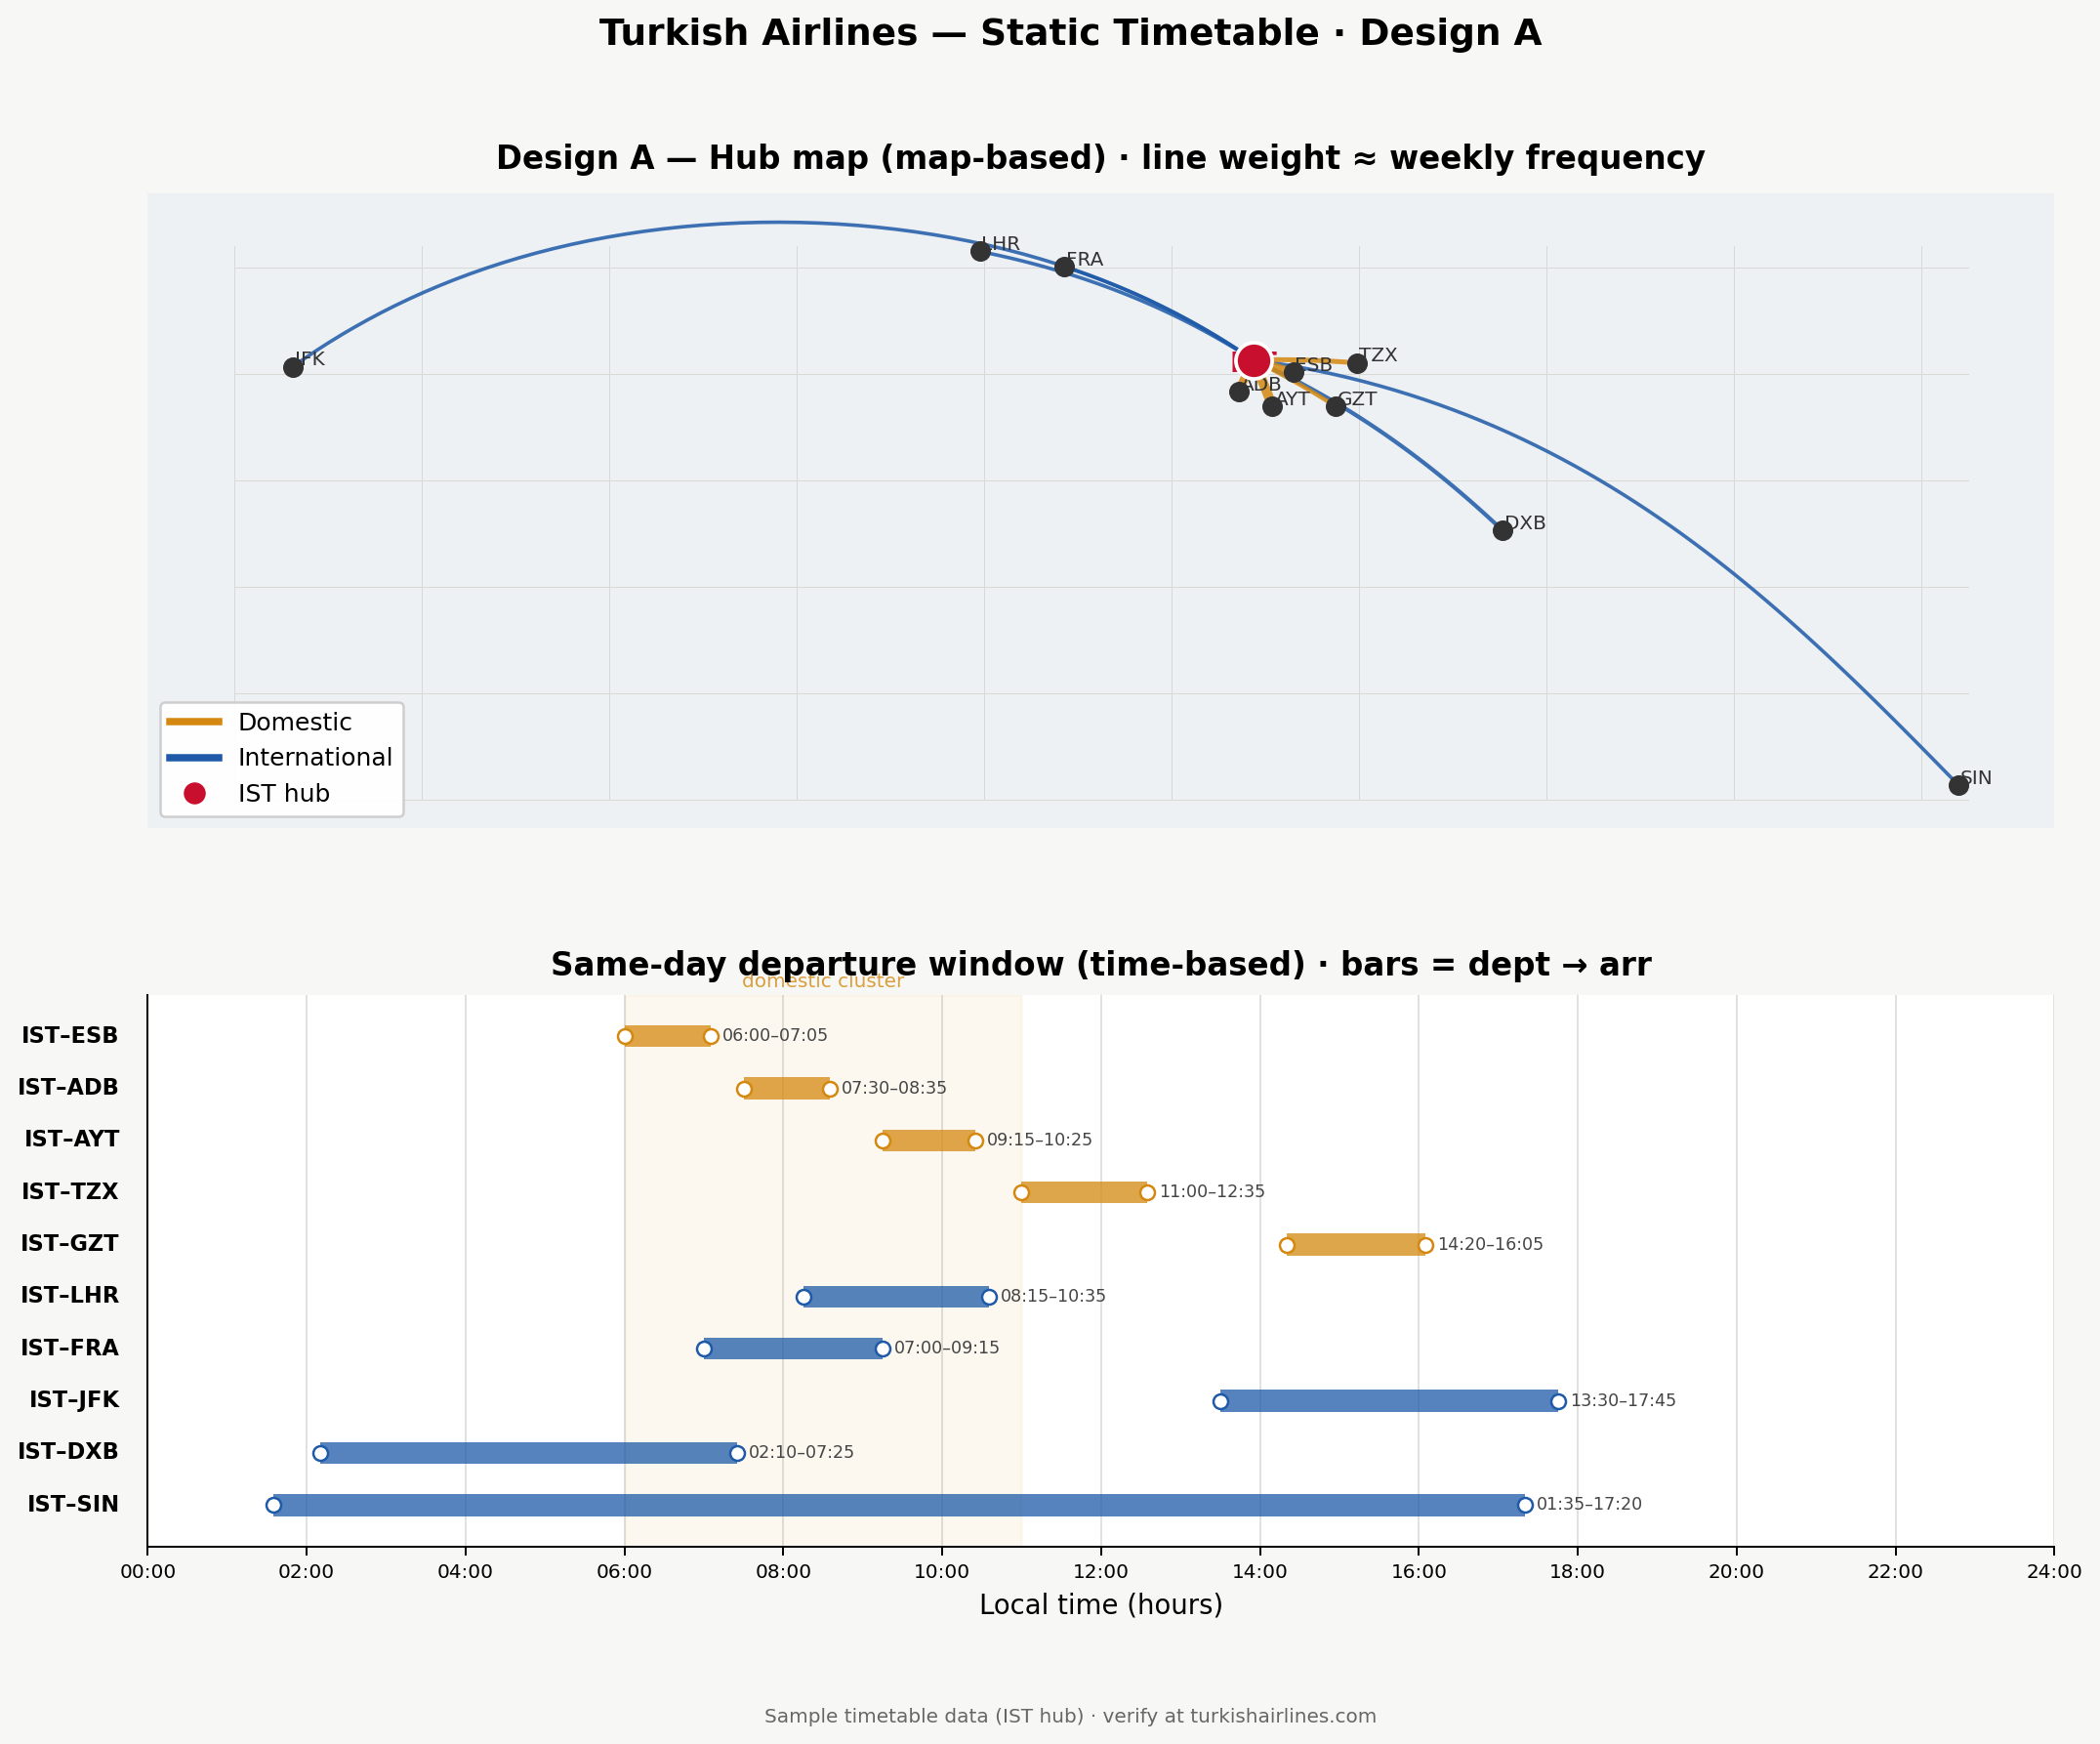
\includegraphics[width=\textwidth]{thy-design-a.png}%
  }{%
    \fbox{\parbox{0.92\textwidth}{\centering\vspace{2.8cm}
    \textbf{[Design A --- insert \texttt{thy-design-a.png}]}\par\vspace{0.4cm}
    \small Hub-and-spoke map (top) + 24-hour departure timeline (bottom)\vspace{2.8cm}}}%
  }
  \caption{Design A: hybrid hub map and same-day departure timeline for ten THY routes.}
  \label{fig:thy-design-a}
\end{figure}

\subsubsection{Gestalt critique (Design A)}

\paragraph{Proximity.}
The map groups arcs that share the IST hub, so all routes read as one network rather than isolated city pairs. On the timeline, bars for the same market (domestic vs.\ international) are placed in adjacent columns, exploiting proximity to suggest category membership. A weakness appears where short domestic bars cluster between 06:00--11:00: their endpoints sit so close that departure times blur unless whitespace or grid lines separate groups.

\paragraph{Similarity.}
Color and stroke weight repeat the same encoding on map and timeline (blue = international, amber = domestic), so similarity carries meaning across panels without a second legend. Bar length on the timeline similarly encodes duration, paralleling longer arcs on the map for intercontinental legs. Where similarity fails, identical bar heights for different routes that share the same duration (e.g., multiple 1h 05m domestic hops) force the reader to read text labels instead of discriminating at a glance.

\paragraph{Continuity.}
The eye can follow an arc from IST outward on the map, then jump to the matching colored bar on the timeline---a deliberate cross-panel continuity aided by shared route labels (IST--LHR, etc.). Continuity breaks for overnight international departures (e.g., IST--SIN at 01:35): the bar wraps past midnight on a single-day axis unless a subtle day-boundary marker is added.

\paragraph{Figure--ground.}
IST is the figure on the map (larger node, saturated fill); landmasses and graticule stay in the ground layer at low contrast. On the timeline, active bars are figure and the 24-hour grid is ground. When too many bars overlap the 06:00--09:00 band, figure--ground inversion occurs and the grid competes with the data---a density problem tied to high domestic frequency.

\paragraph{Closure.}
Readers mentally close each arc into a full great-circle path even where only a chord is drawn---useful for geographic reasoning. On the timeline, paired departure and arrival ticks invite closure into a complete ``trip interval,'' though multi-segment or overnight flights need explicit break markers so closure does not imply a same-calendar-day arrival incorrectly.

\paragraph{Summary.}
Design~A unifies space and time but risks morning-cluster clutter on the timeline. Gestalt grouping is strongest when map color, label, and bar share one route identity; weakest where temporal overlap and short domestic durations collapse distinct flights into one visual band.

%------------------------------------------------------------------------------
\subsection{Design B: Route strip map with vertical schedule column}
%------------------------------------------------------------------------------

\textbf{Layout.} A \textbf{map-based} strip (left third) uses a simplified east--west band: Turkey enlarged, with straight segments from IST to each domestic city and curved segments to international destinations. A \textbf{time-based} column (right two thirds) lists routes vertically; each row holds a mini 06:00--24:00 scale with a dot for departure and a second dot for arrival, connected by a horizontal segment whose length is proportional to block time. Weekly frequency appears as repeated tick marks under the row label.

\begin{figure}[H]
  \centering
  \IfFileExists{images/thy-design-b.png}{%
    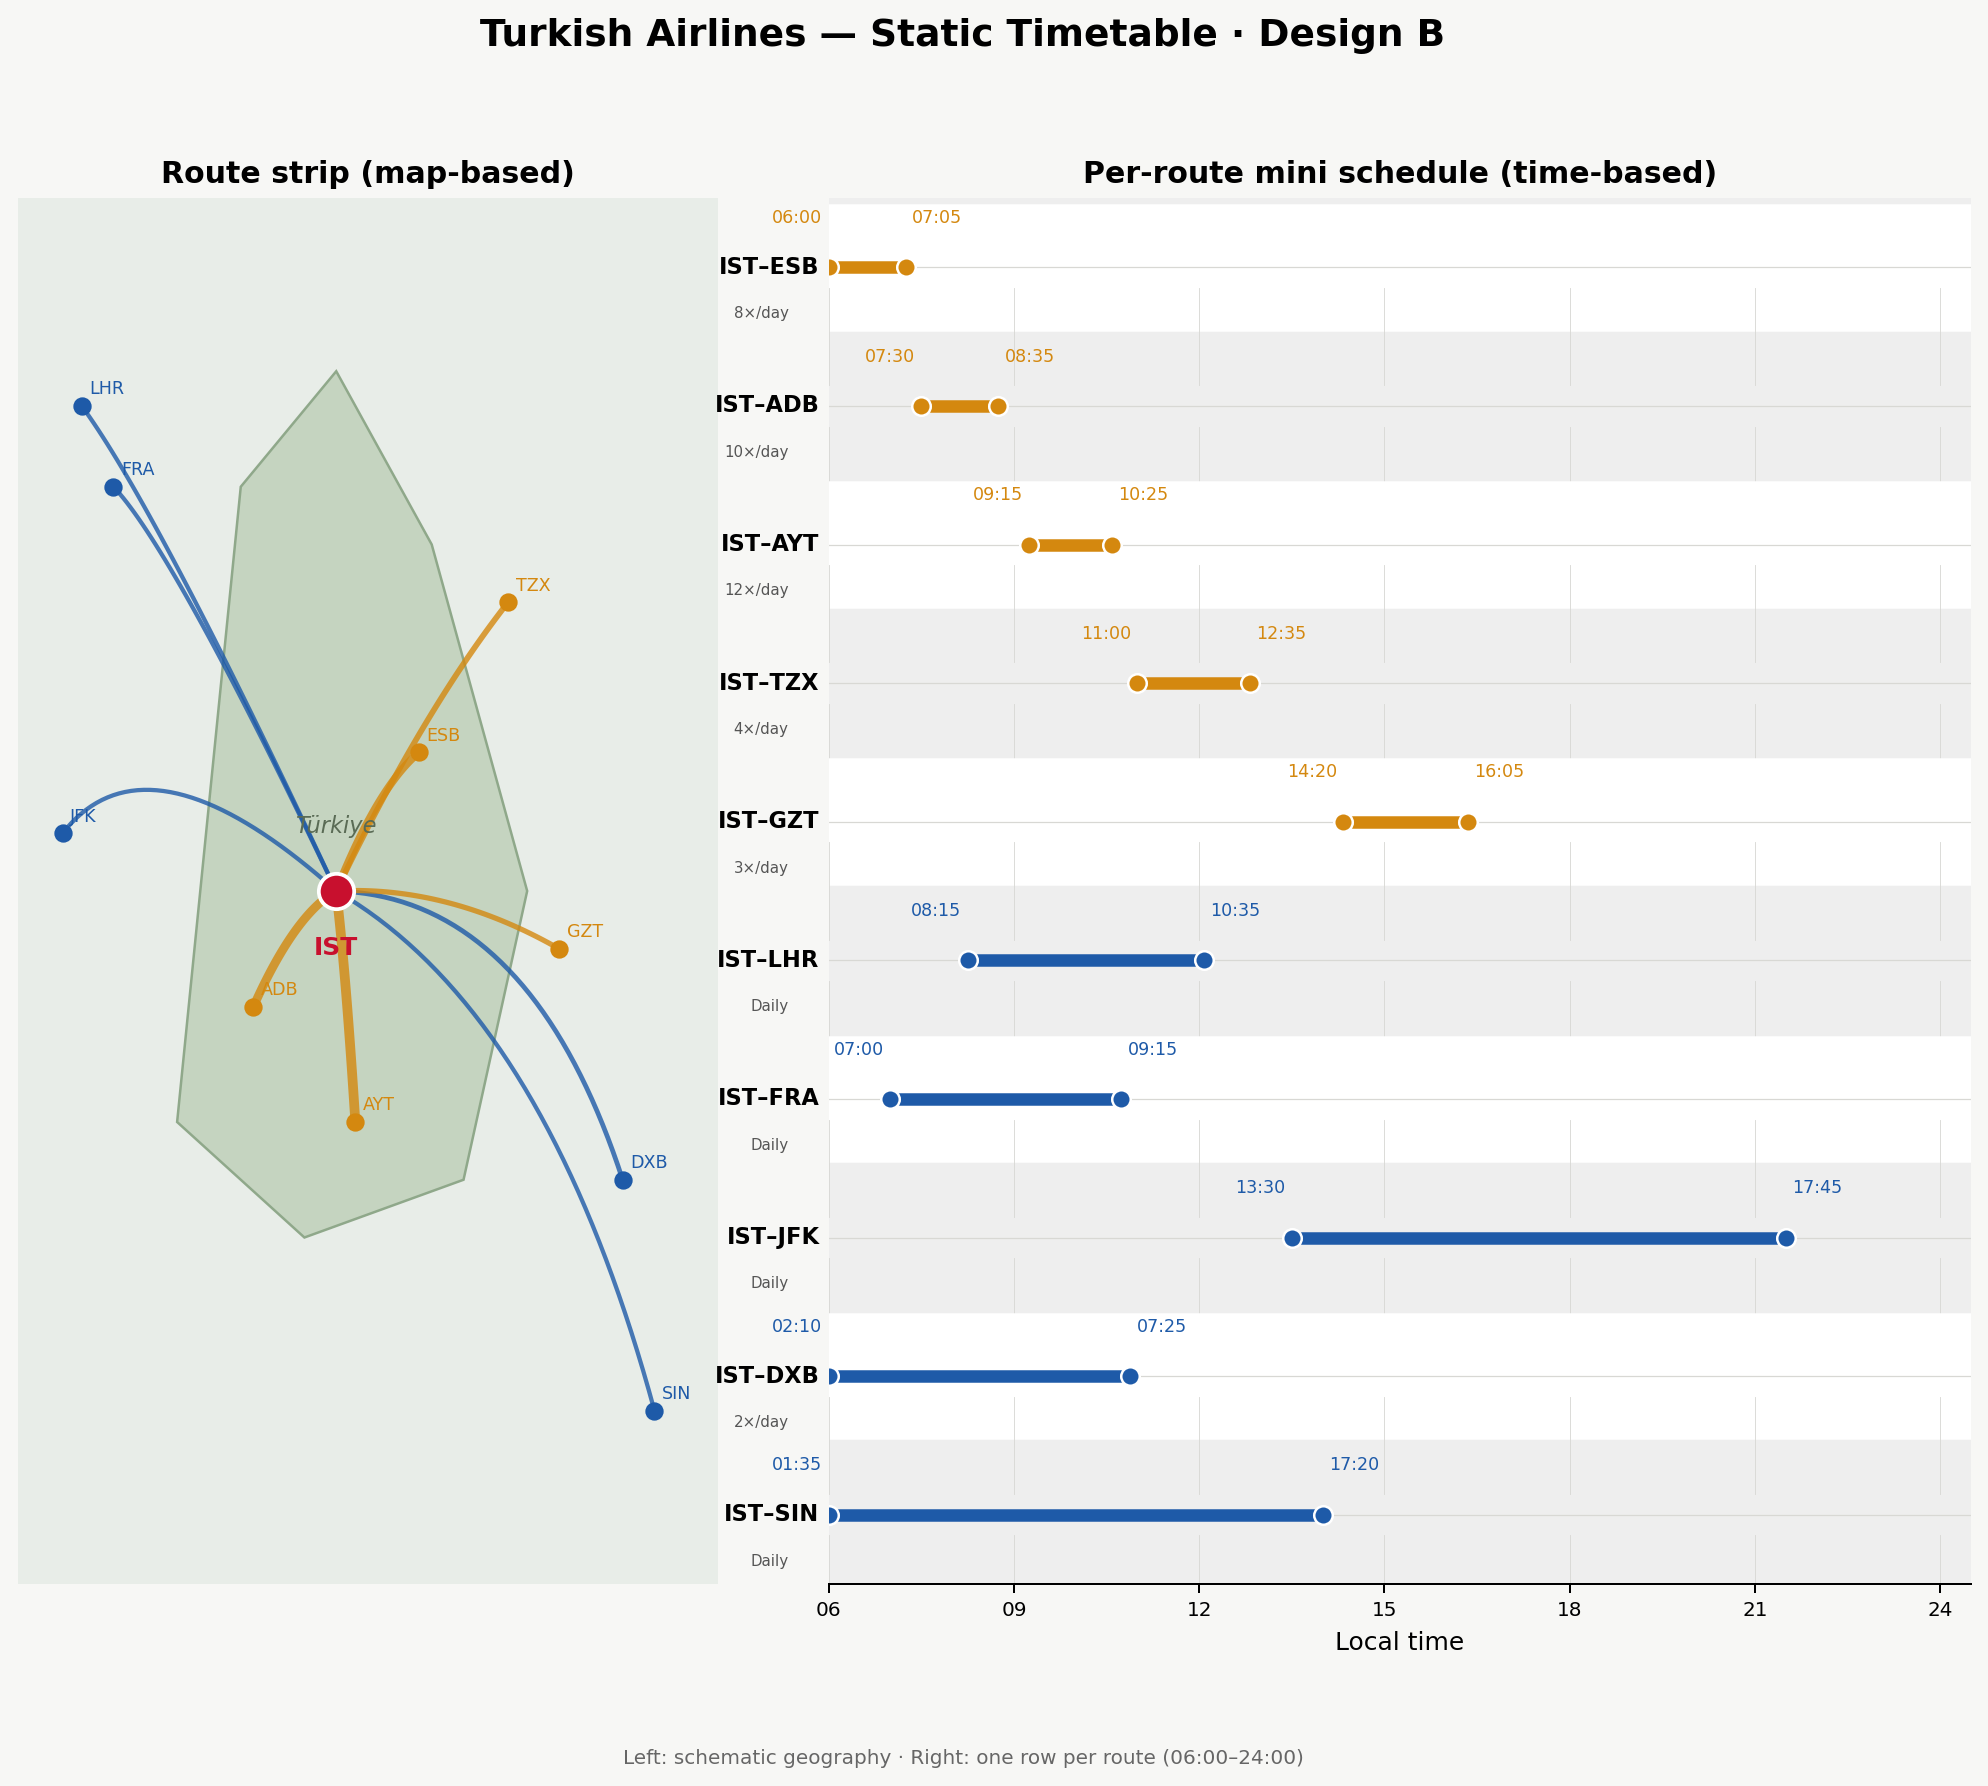
\includegraphics[width=\textwidth]{thy-design-b.png}%
  }{%
    \fbox{\parbox{0.92\textwidth}{\centering\vspace{2.8cm}
    \textbf{[Design B --- insert \texttt{thy-design-b.png}]}\par\vspace{0.4cm}
    \small Geographic route strip (left) + vertical per-route time scales (right)\vspace{2.8cm}}}%
  }
  \caption{Design B: route strip map paired with vertical mini-timelines per route.}
  \label{fig:thy-design-b}
\end{figure}

\subsubsection{Gestalt critique (Design B)}

\paragraph{Proximity.}
Each route occupies one horizontal band in the schedule column, so departure dot, segment, and arrival dot are proximate and read as one object. Domestic rows are stacked above international rows, using vertical proximity as a secondary filter. Proximity fails on the map strip when European and Middle Eastern international destinations compress: segment endpoints crowd the IST--Anatolia corridor and labels must float outward, weakening the link between name and geography.

\paragraph{Similarity.}
All rows share the same mini-scale grammar (dot--line--dot), so once learned, the schema applies to every route---strong similarity for learnability. Frequency tick marks under labels reuse the same stroke, differing only in count. Similarity becomes a weakness when JFK and SIN rows both use long segments on different absolute scales: without a row-specific time-axis label, similar shapes can imply comparable \emph{clock} spans even when one row is stretched for legibility.

\paragraph{Continuity.}
Vertical reading down the schedule follows the airline's operational list logic (check one route, move to the next). The map strip encourages left-to-right continuity from hub to spoke. Continuity across panels requires matching route codes on left and right; if labels align only by color, a color-blind reader loses the bridge---continuity should be reinforced with text anchors, not color alone.

\paragraph{Figure--ground.}
The schedule column uses white rows on a light gray field so each route band is figure. On the strip map, only route segments and city dots are figure; simplified coastlines remain ground. Long international segments that cross the strip diagonally sometimes dominate the figure layer and obscure shorter domestic spokes---a figure--ground imbalance that favors long-haul routes visually even when domestic frequency is higher.

\paragraph{Closure.}
Mini-timelines invite closure between departure and arrival ticks as a single ``flight envelope.'' The map strip allows closure of IST as the hub that completes the network star, even when segments do not physically meet at one point on the simplified basemap. Closure misfires for routes with large time-zone shifts if the mini-scale is always local time without a time-zone glyph: the reader may close the segment as a single time zone incorrectly.

\paragraph{Summary.}
Design~B scales well to ten routes by giving each its own temporal row, reducing overlap compared with Design~A's shared 24-hour axis. Gestalt strengths are row-wise proximity and repeated mini-scale similarity; primary risks are map-strip crowding near IST and ambiguous cross-panel linkage if labels and color are not redundant.

%==============================================================================
\section{Part 3: Interactive Timetable Dashboard}
%==============================================================================

The interactive prototype is a single-page web dashboard (\texttt{thy-dashboard.html}) built with Plotly.js. It reuses the ten IST hub routes from Part~2 and organizes the interface around \textbf{Shneiderman's mantra}: an overview of the full network first, linked filters and zoom/pan second, and a detail panel on demand when the user selects a route.

\begin{figure}[H]
  \centering
  \includegraphics[width=\textwidth]{{dashboard2.png}}
  \caption{Interactive dashboard UI: summary cards and hub map (overview), sidebar filters and departure timeline (filter), empty detail panel until a route is selected (details on demand).}
  \label{fig:thy-dashboard}
\end{figure}

\subsection{Interface structure}

\textbf{Overview.} Four summary cards report total, filtered, international, and domestic route counts. The central \emph{network map} shows great-circle arcs from IST; line weight and color encode route type (blue = international, amber = domestic). The lower \emph{departure timeline} lists the same routes as horizontal bars on a 24-hour axis so temporal clustering---especially morning domestic departures---is visible at a glance.

\textbf{Filter and zoom.} The left sidebar filters by route type, destination city, and local departure window. Map zoom and pan use Plotly's default geo controls; \emph{Fit map view} recenters the projection. The route list mirrors filtered results and supports keyboard-free selection.

\textbf{Details on demand.} Clicking a map marker, timeline bar, or list item fills the right panel with origin, destination, local times, block time, frequency, and aircraft---without cluttering the overview.

\subsection{Reflection (Part 3)}

The dashboard works best when the user needs a \emph{mental model} of the hub network before reading exact times. The map overview immediately communicates IST centrality and the geographic stretch of long-haul legs (JFK, SIN) versus short domestic spokes (ESB, ADB). Linking map color to timeline bar color preserves continuity across views: once learned, the encoding transfers without a second legend. Summary cards give honest feedback after filtering (\emph{visible after filter}), which supports exploratory analysis and satisfies the ``overview first'' step even after the dataset is subset.

Several failures appeared in testing. The clearest \textbf{failure case} is narrowing the departure window to morning hours (e.g., 06:00--10:00) while leaving route type on \emph{All}: international overnight departures (IST--SIN at 01:35, IST--DXB at 02:10) vanish from the timeline, but their map arcs can remain visually prominent until the map is redrawn, momentarily suggesting routes that are filtered out of the schedule view. A second failure occurs when many domestic bars overlap between 07:00 and 10:00: bars share similar length (about one hour), so users must read labels rather than discriminate by shape---the same similarity problem noted in static Design~A. Finally, the detail panel stays empty until click; first-time users sometimes did not discover it, treating the dashboard as view-only.

\textbf{Trade-offs} are inherent in a single HTML file without a backend. We favored linked brushing (map, timeline, list, detail) over showing every daily frequency instance: the data represent sample departures, not a full weekly matrix, which keeps the UI readable but limits operational use. Local times are shown without time-zone badges, so block times on intercontinental routes can be misread as single-zone intervals---acceptable for a class prototype, misleading for trip planning. Plotly's geo projection also compresses Europe and the Middle East, echoing Part~1B's hub-crowding problem in digital form.

One \textbf{design decision changed after testing}. Initially, each filter change fully rebuilt the map with \texttt{Plotly.newPlot}, which reset zoom and pan---frustrating users who had drilled into Southeast Asia and then adjusted the departure slider. We switched to \texttt{Plotly.react} for updates after the first render so the viewport persists unless \emph{Fit map view} is pressed. That small change aligned the implementation with Shneiderman's ``zoom'' step: filtering should refine the overview, not destroy spatial context.

\textbf{Improvements} for a production version would include: synchronized highlight on filter (dim non-matching arcs immediately); per-route frequency layers or a ``show all departures'' toggle; explicit time-zone labels in the detail panel; and mobile layout stacking (sidebar below map on narrow screens). Despite these limits, the dashboard demonstrates that interactivity recovers some spatial reasoning lost in print timetables while still requiring careful encoding when many similar short flights share the same morning band.

\noindent\textit{Interactive file:} \texttt{thy-dashboard.html} (open in any modern browser with network access for the Plotly CDN).

\end{document}
